\documentclass{article}

% Language setting
% Replace `english' with e.g. `spanish' to change the document language
\usepackage[spanish]{babel}

% Set page size and margins
% Replace `letterpaper' with `a4paper' for UK/EU standard size
\usepackage[a4paper,top=2cm,bottom=2cm,left=3cm,right=3cm,marginparwidth=2cm]{geometry}

% Useful packages
\usepackage{amsmath}
\usepackage{parskip}
\usepackage{graphicx}
\usepackage[colorlinks=true, allcolors=black]{hyperref}
\usepackage{fancybox}
\usepackage{listings}
\usepackage{subcaption}
%\lstset{
%    language=Matlab,
%    extendedchars=true
%}
\setlength{\parskip}{0pt}

\title{Comportamiento del protocolo Aloha Ranurado}
\author{Álvaro Hernández Riquelme}
%\date{}

\begin{document}
\maketitle

\tableofcontents
\newpage

%\begin{abstract}
%Your abstract.
%\end{abstract}


\section{Introducción al trabajo}

Para este trabajo, se estudiará el comportamiento de un protocolo de Aloha Ranurado usando un sistema SDL, donde se completará la edición, simulación y validación total del protocolo. Tras esto, se hará un estudio de éste.

\quad

\textbf{SDL}, también conocido como Simulation and Description Language, es el lenguaje de especificación formal creado por la ITU para definir y representar sistemas y protocolos. Se usará la herramienta \textbf{Telelogic Tau}, para representar nuestra especificación de \textbf{Aloha Ranurado}. Tendremos una base sin terminar del protocolo en el aula virtual, la cual modificaremos y completaremos, finalmente haremos una simulación y validación. 

\quad

\textbf{Aloha} es un protocolo de acceso al medio aleatorio, donde varios nodos pueden compartir información con una probabilidad de colisión, ya que se envía la información sin comprobar si el canal está libre. Quiere decir que si en el tiempo de envío, existe otro nodo transmitiendo, se producirá ésta colisión. Para mejorar las prestaciones, se define \textbf{ALOHA ranurado}, donde se dividen las transmisiones de mensajes en slots del tamaño de éste mensaje y los nodos solo pueden transmitir al inicio de los slots. De este modo, se reduce el periodo de colisión.

\subsection{Nuestro Entorno}

Como se ha dicho previamente, usaremos Telelogic Tau para la simulación del protocolo. Al abrirlo, si cargamos la base del trabajo proporcionada en el aula virtual, podremos empezar a trabajar sobre ésta.

\quad

\begin{figure}[h]
    \centering
    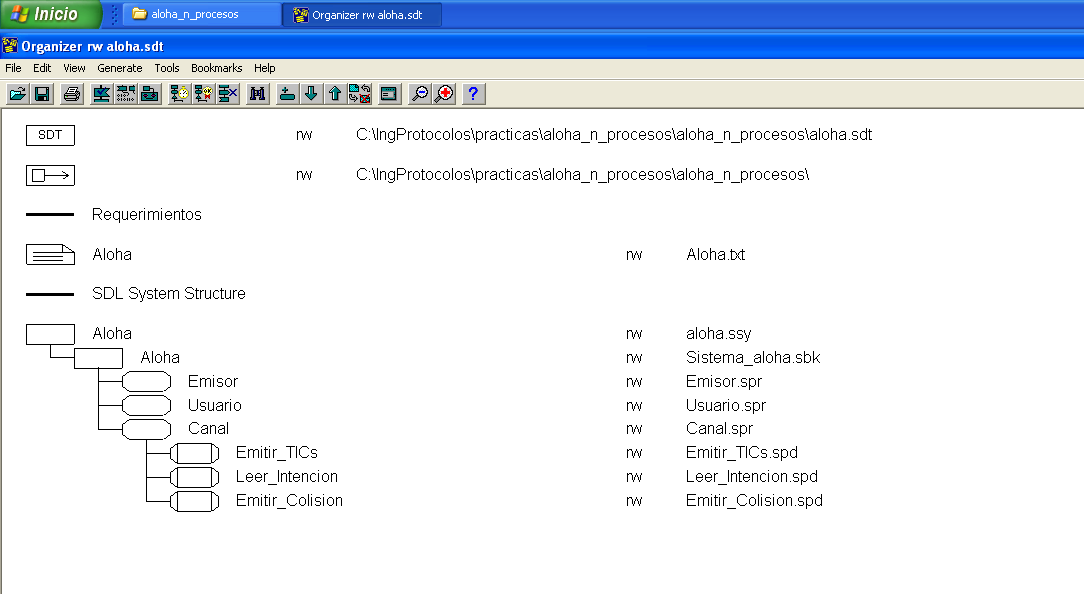
\includegraphics[width=1\linewidth]{src/Organizer-tltau.png}
    \caption{\label{fig:tltau} Inicio de Telelogic Tau con el proyecto de ALOHA Ranurado.}
\end{figure}

\newpage

\section{Edición}

Como se nos ha comentado en clase, antes de ir a la simulación y validación, tendremos que emepzar con la edición, ya que la base proporcionada no está completa. Teniendo en cuenta la captura anterior, y usando el programa para ver qué hay hecho, vemos que los procesos \textbf{Emisor, Usuario, y Canal} están sin terminar, por lo que empezaremos diseñando estos estados.
Es importante reconocer qué significa cada símbolo:

\begin{figure}[h]
    \centering
    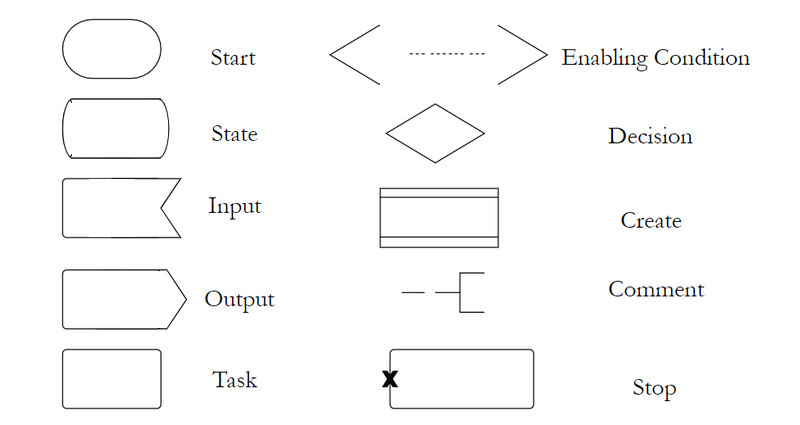
\includegraphics[width=0.7\linewidth]{src/sdl-symbols.jpg}
    \caption{\label{fig:sdlsymbols} Significado de los símbolos en SDL.}
\end{figure}

\quad

\subsection{Emisor}

Para el bloque \textbf{emisor}, crea su correspondiente instancia de proceso usuario, entonces le damos a user el valor de \verb|Offspring|,  que es una variable del sistema que nos permitirá asignar una ID a cada usuario. Una vez esto, el usuario puede que tenga un mensaje que transmitir o no. Dependiendo irá por una rama o por otra. 

\begin{figure}[h]
    \centering
    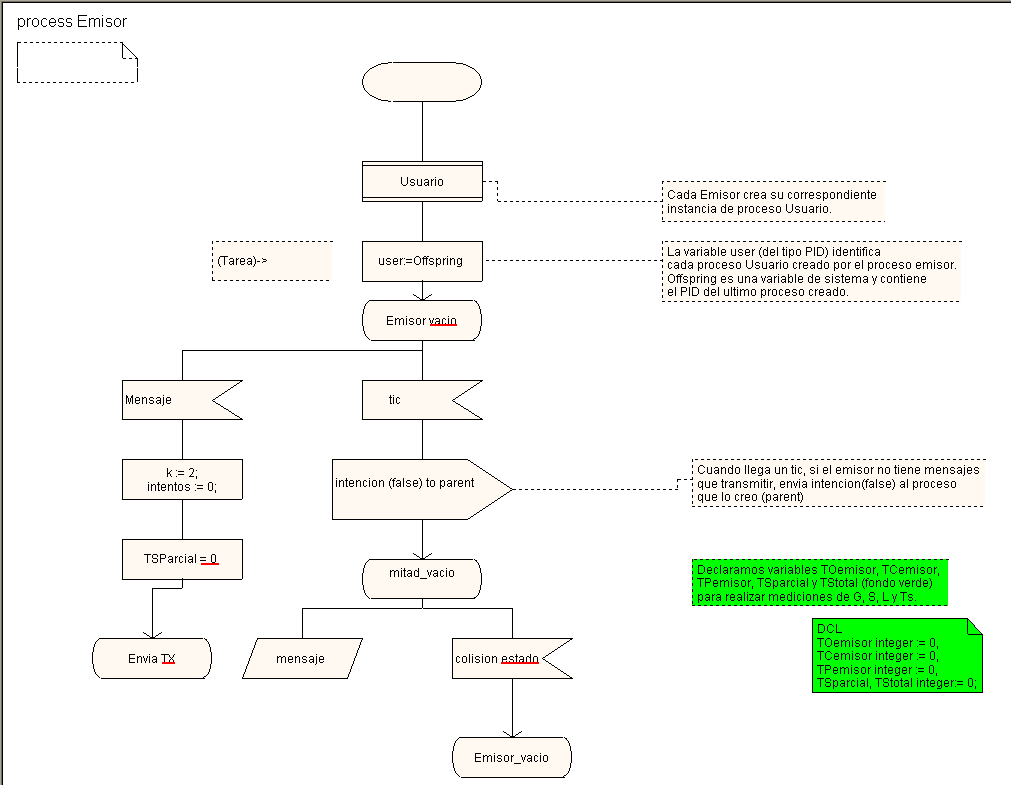
\includegraphics[width=0.8\linewidth]{src/Estado emisor.png}
    \caption{\label{fig:emisorbl} Diagrama del proceso emisor.}
\end{figure}

Vemos que al iniciar el emisor, en el momento que llega a \verb|Emisor vacío|, espera 2 tipos de inputs: mensaje o tic. En caso de que haya un mensaje que transmitir, va a la izquierda, donde asignamos una k y reseteamos los intentos para transmisión y el tráfico parcial. Iríamos al estado \verb|Envía TX|. En cambio, si no hay un mensaje que transmitir, recibiríamos un tic, donde se envía la intención de que efectivamente no queremos transmitir a quien lo creó y, en caso de que haya un mensaje para transmitir se guardaría para el siguiente tic y si no, iríamos de vuelta al estado \verb|Emisor vacío|. 

\subsubsection{Estado Envia TX}

El estado empieza esperando a recibir el input del próximo tic, al pasar, aumentaremos en 1 las variables de TOemisor y TSparcial. En este caso, en vez de enviar la intención de que \textbf{no} queremos envíar, envíamos que \textbf{sí} querríamos, con un true. Al entrar al estado \verb|ficticio|, comprobamos con el input de estado, si existe colisión o no, por lo que si no hubiera, el proceso \verb|Emisor| crearía un \verb|Usuario| (envía true a usuario). en caso contrario, se aplicaría el algoritmo backoff un número máximo de reintentos como mucho, siendo que si no lo conseguimos finalmente, no se enviaría el resultado true a \verb|Usuario|.
Vemos el diagrama de \verb|Envía TX|:

\quad

\begin{figure}[h]
    \centering
    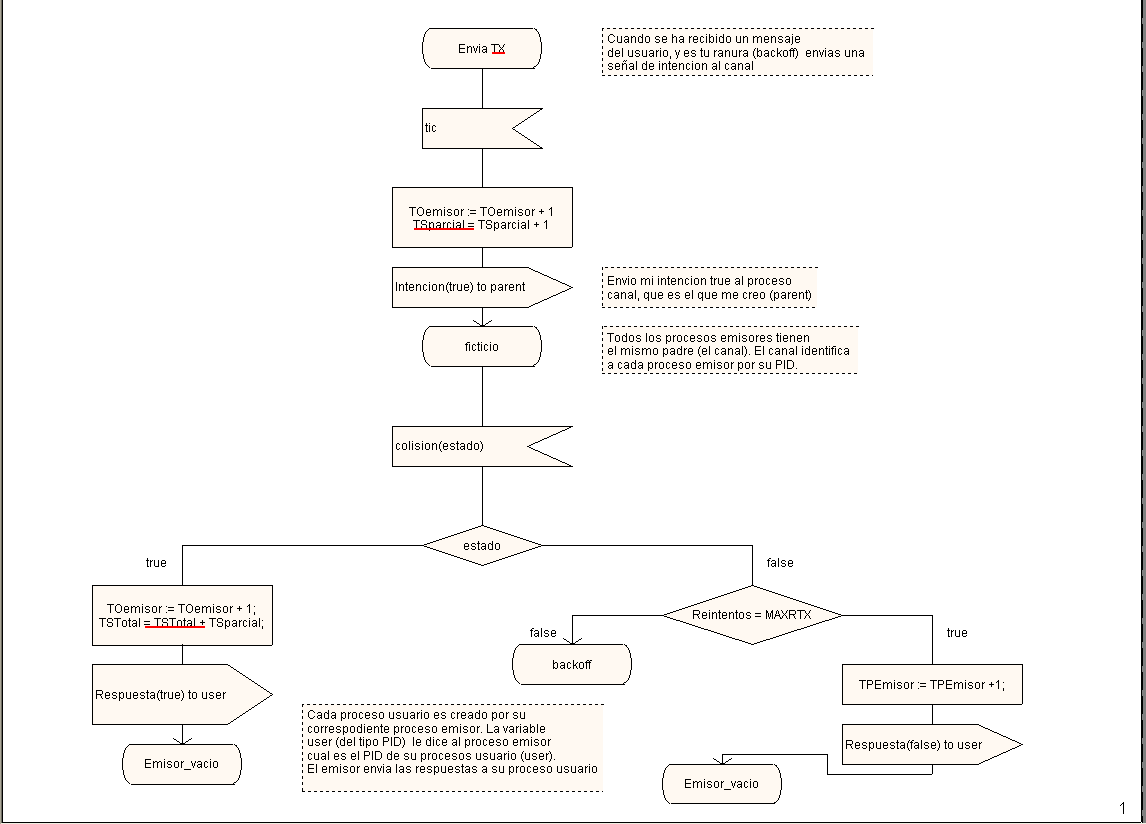
\includegraphics[width=0.8\linewidth]{src/Estado enviatx.png}
    \caption{\label{fig:enviatxbl} Diagrama del estado Envia TX.}
\end{figure}



\subsubsection{Algoritmo Backoff}

Como hemos visto antes, es posible que en el estado haya una colisión al intentar transmitir el mensaje, es por eso que si el estado de colisión nos devuelve \textbf{false}, y no nos hemos pasado el límite de intentos, iremos al algoritmo \verb|backoff|.

En este estado, simplemente generaremos un número aleatorio \textbf{k} de ranuras, y las iremos reduciendo en cada tic hasta llegar a 0, donde llegaría el turno de enviar otra vez, e intentaríamos de nuevo enviar volviendo al estado \verb|Envía TX|, podría ser que se envíe tras el estado, o que vuelva a haber colisión, se generaría un bucle hasta que no haya colisión o no supere el máximo de intentos.
\newpage

\begin{figure}[htb]
    \centering
    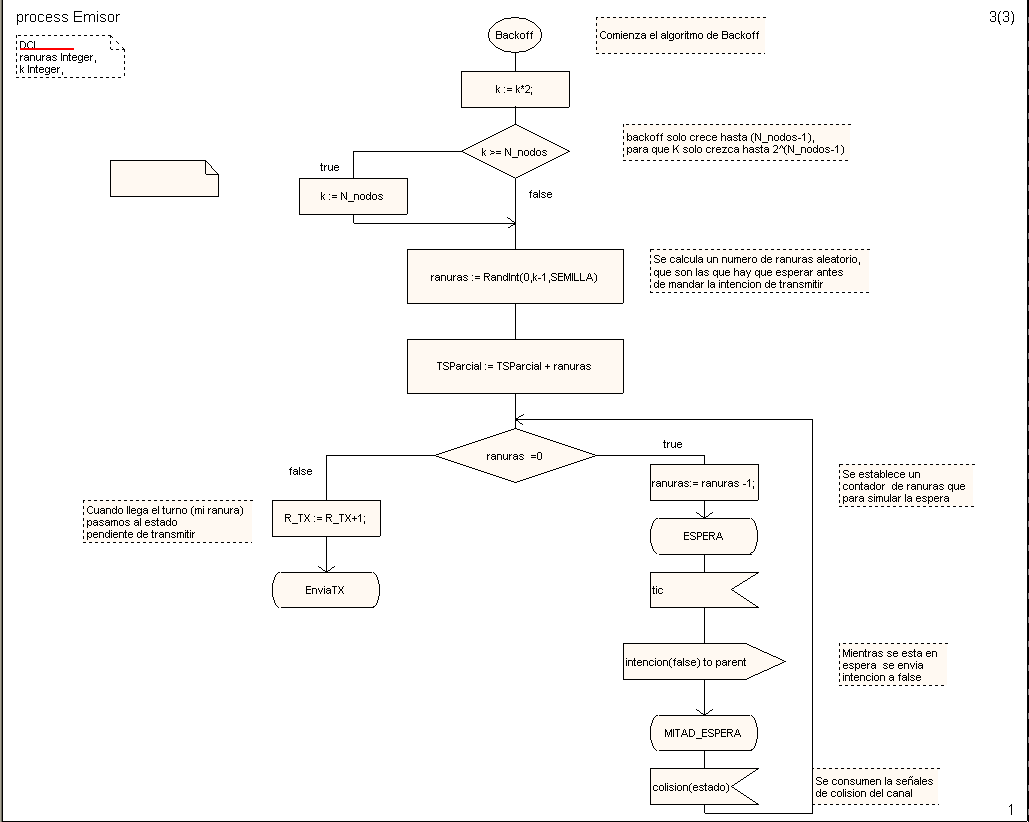
\includegraphics[width=0.85\linewidth]{src/backoff state.png}
    \caption{\label{fig:backoffstate} Diagrama del Algoritmo Backoff.}
\end{figure}

\quad

\subsection{Usuario}

El proceso usuario nos indicará si existe una intención de transmitir o no. Será el encargado de enviárselo al emisor. Consistirá en una probabilidad Pg donde puede \textbf{enviarse o no. (true o false)}

\quad

\begin{figure}[h]
    \centering
    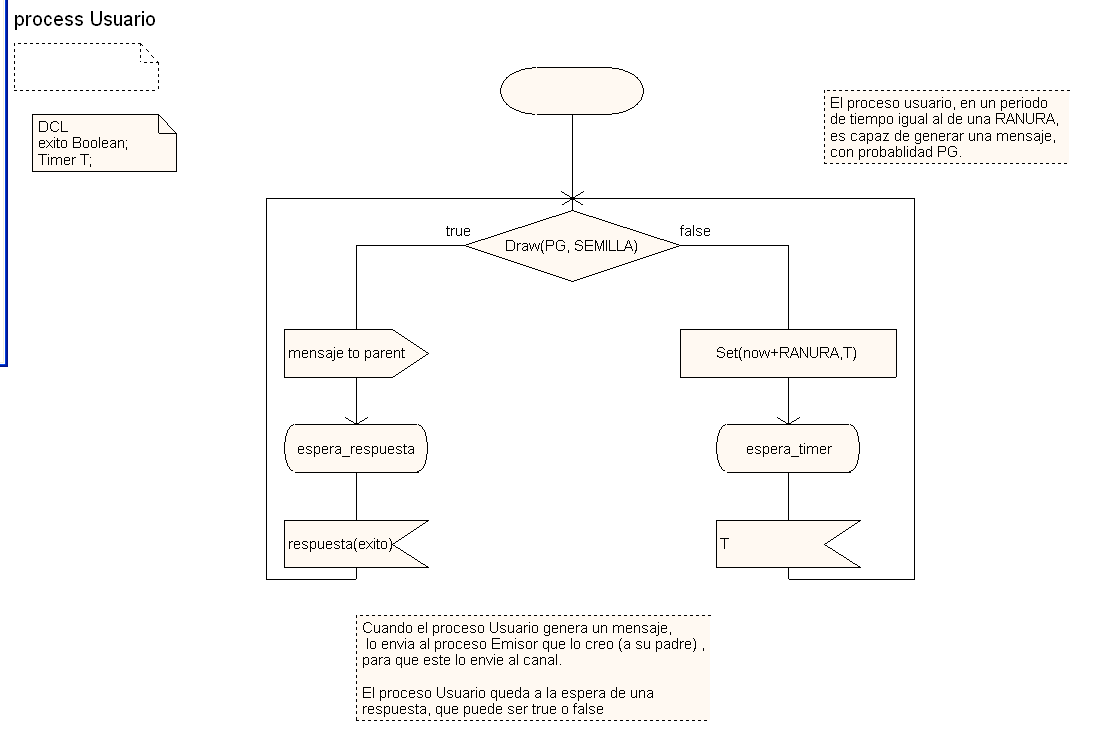
\includegraphics[width=0.7\linewidth]{src/captura usuario.png}
    \caption{\label{fig:usuariodiagr} Diagrama del proceso Usuario.}
\end{figure}

\quad

Cabe destacar que, tal como nos indicaba el manual sobre ALOHA, debíamos insertar la función set, teniendo como parámetro de "\(\)Expr " \textbf{RANURAS}, y de "TimerName" \textbf{T}.
\subsection{Canal}

El canal se encarga de mantener la estabilidad y organización del sistema, esto es, debido a que lleva el conteo de tics (Como si fuera el clk) y a la vez con los procedimientos \verb|Leer intención| y \verb|Emitir colisión| comprobaremos si existe colisión y se lo comunicaremos a los demás procesos.

\quad

Entonces, finalmente en la captura veremos que este proceso termina en un "bucle" donde generamos un tic, y según las intenciones emitiremos una colisión o no:

\begin{figure}[h]
    \centering
    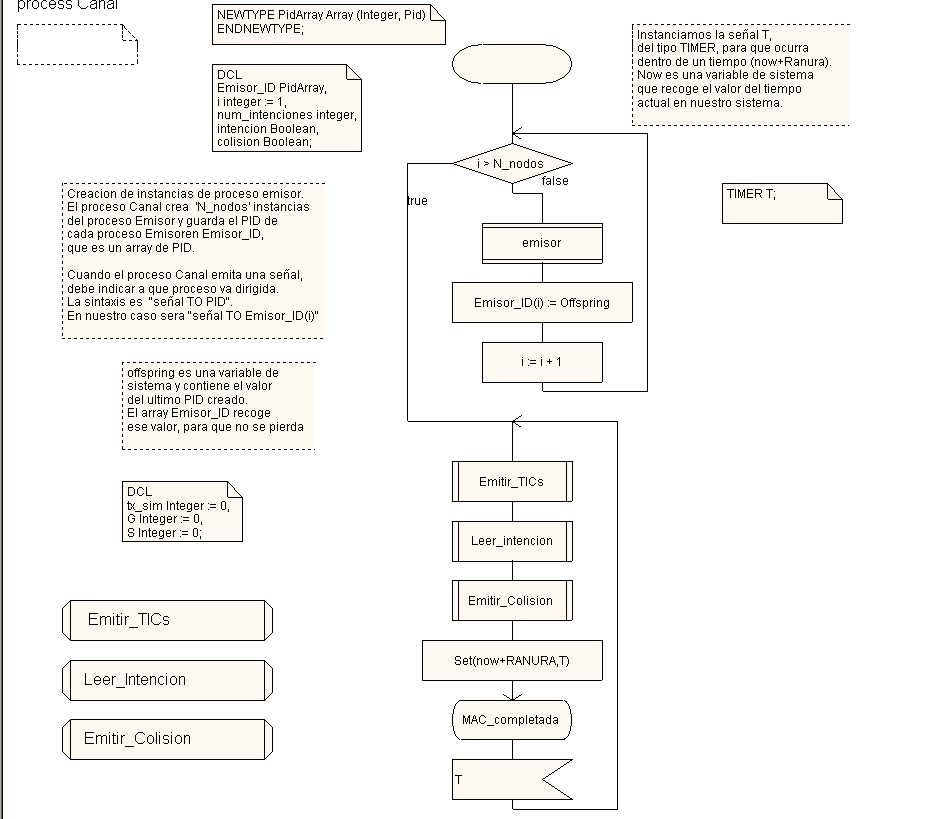
\includegraphics[width=0.8\linewidth]{src/proceso canal.png}
    \caption{\label{fig:canalproceso} Diagrama del proceso del canal.}
\end{figure}


En el proceso de canal, tendremos tres procedimientos: \textbf{emitir tics}, \textbf{leer intención}, y \textbf{emitir colisión}:

\subsubsection{Emitir Tics}

Éste procedimiento, únicamente lo que hará será tener un contador que será  incrementado cada vez que se le llama, y a la vez se lo enviará como Output al \verb|Emisor| , como vemos en \textbf{tic to Emisor id i}

\begin{figure}[hbt]
    \centering
    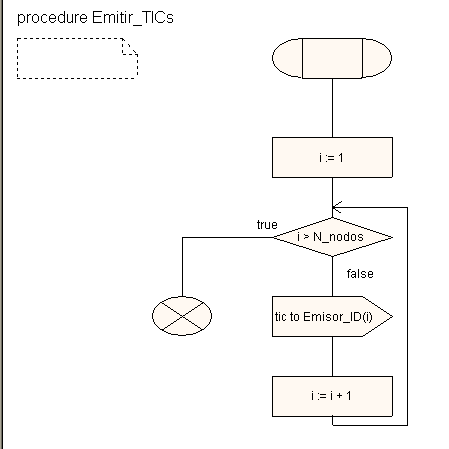
\includegraphics[width=0.3\linewidth]{src/proc emitir tics.png}
    \caption{\label{fig:emitirtics} Procedimiento emitir tics.}
\end{figure}

\subsubsection{Leer Intención}

El procedimiento leer intención, recibirá el input de intención, y dependiendo de si hay intención o no, (true o false), se incrementará la variable num intenciones o i.

\quad

\begin{figure}[h]
    \centering
    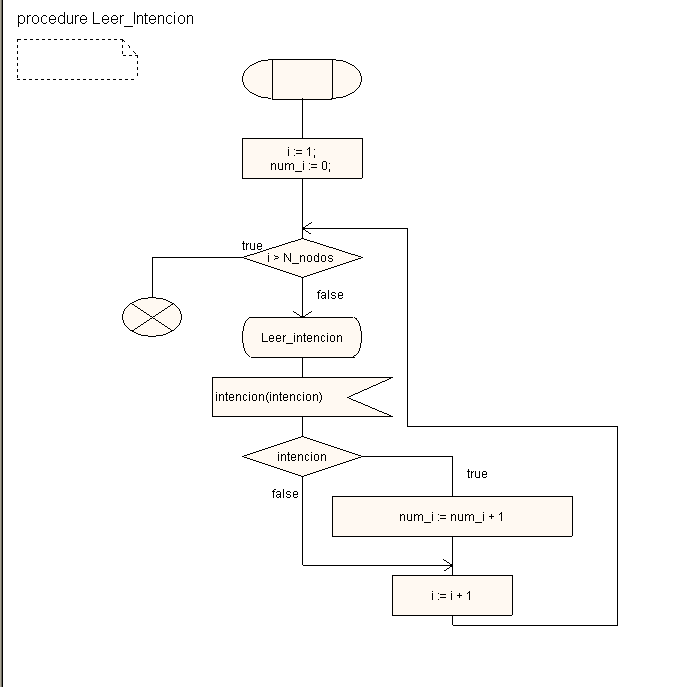
\includegraphics[width=0.6\linewidth]{src/leer intencion.png}
    \caption{\label{fig:leerintencion} Procedimiento leer intencion.}
\end{figure}

\subsubsection{Emitir colisión}

En el procedimiento de leer intención hemos visto, que si hay intención de transmitir, incrementaremos 1 en la variable num intenciones. En este caso, en emitir colisión, usaremos esta variable para confirmar si existe o no una colisión, y emitirla en caso afirmativo. Ésto pasaría, cuando la variable num intenciones es mayor que uno (Más de una intención de transmitir en el canal), en este caso pondríamos colisión en \textbf{True.}

\quad

\begin{figure}[h]
    \centering
    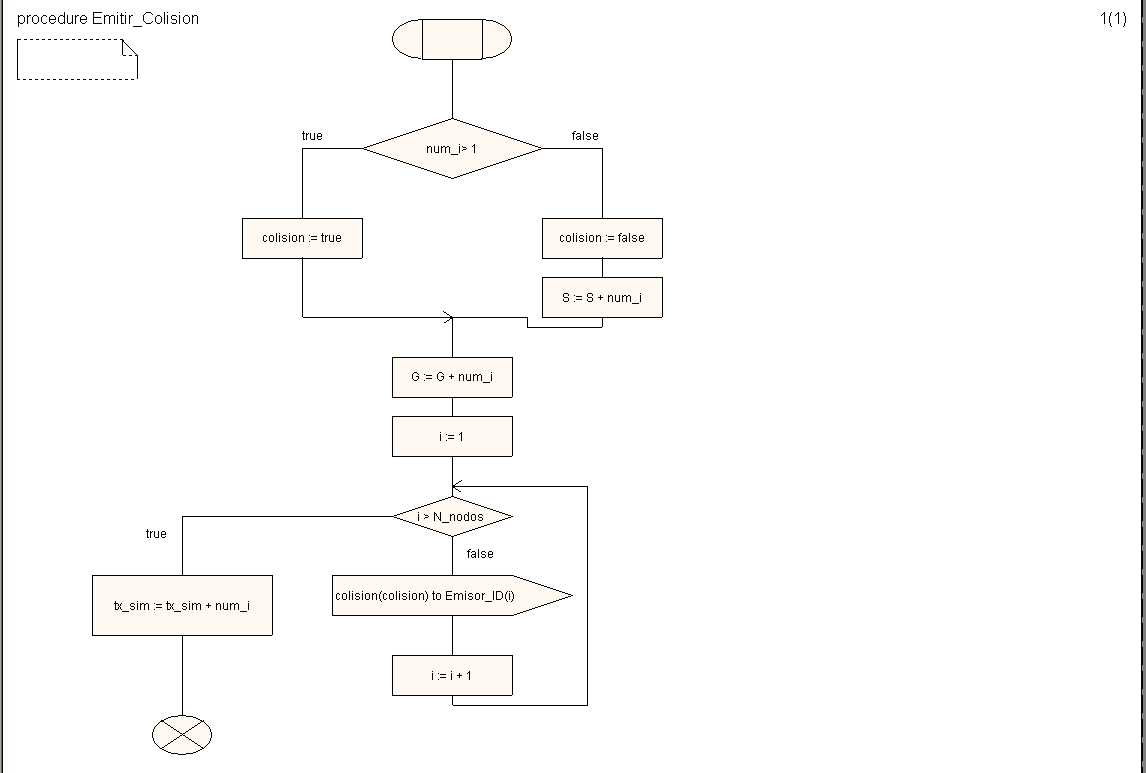
\includegraphics[width=0.8\linewidth]{src/proc emitir col.png}
    \caption{\label{fig:emitircol} Procedimiento emitir colisión.}
\end{figure}
\newpage

\section{Validación}

La parte de validación consiste en la confirmación del funcionamiento y posible detección de errores del sistema. Específicamente, validaremos el comportamiento del sistema SDL. En este caso, se seguirán los pasos incluidos por el tutorial para la validación de éste, junto a otros usados en el tutorial del Demongame.

\quad

\subsection{Validación manual}

Iniciaremos el validador mediante las formas usadas en clase y los tutoriales, en las que se asumirá algunas partes ya conocidas, o se explicará con menos detalle al no ser tan relevantes el funcionamiento. Empezaremos yendo a \textbf{generate} $\rightarrow$ \textbf{make} $\rightarrow$ \textbf{fullmake}, habiendo seleccionado el standard kernel \textbf{Microsoft Validation}. De este modo, se nos habrá creado un archivo \textbf{Aloha}\verb|_|\textbf{vlc.exe}, tras abrir el validator UI, tendremos que abrir este archivo .exe, y podremos proceder a la validación.

\quad

% El comando \verb|_| es debido a que no se puede añadir una barra baja en LaTex solamente.
Una vez abierto, nos preguntará sobre las variables externas PG y N\verb|_|nodos, donde PG lo marcaremos en 0.95 y N\verb|_|nodos será marcado por el valor que nos avisan en el aula virtual este curso, que será de 7.

\begin{figure}[h]
    \centering
    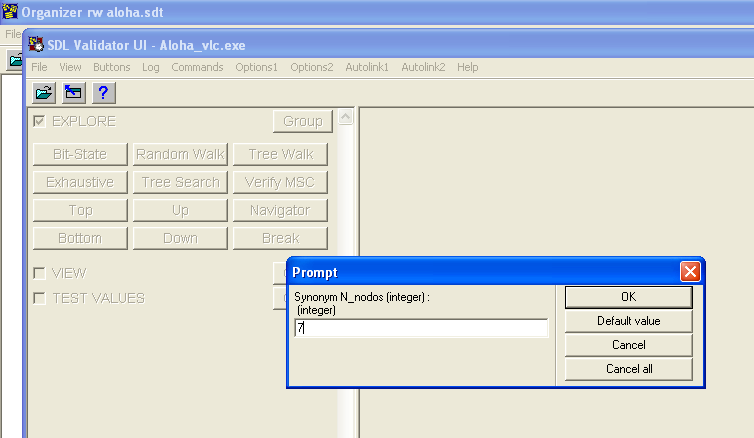
\includegraphics[width=0.80\linewidth]{src/variable 7nodos.png}
    \caption{\label{fig:simulador7nodos} Selección de los 7 nodos al inicio de la validación.}
\end{figure}

\subsection{Árbol de comportamiento}

En el árbol de comportamiento exploramos el sistema de estados del sistema navegando manualmente. El Validador se comportará de manera similar al Simulador, pero con alguna diferencia, por ejemplo trabajaremos con el espacio de estados lo más pequeño posible. Una transición entre dos estados se corresponde a una transición completa en el sistema SDL. 

\begin{figure}[h]
    \centering
    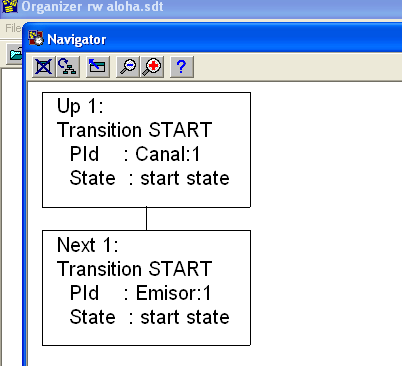
\includegraphics[width=0.35\linewidth]{src/arbol estados.png}
    \caption{\label{fig:arbolestados} Transición en el árbol de estados.}
\end{figure}


Abriremos el árbol de comportamiento donde podremos navegar por los estados, y comprobaremos que representa el funcionamiento del aloha que hemos montado anteriormente, podemos observar el inicio de transición de canal, tras eso crea los procesos de emisor, y seguirá en orden si no se encuentra error. 

Si seguimos los estados, llega un momento que encontramos un error en la creación del emisor 4, que nos hará imposible seguir las transiciones, nuestro error tendrá el mensaje:

\quad

\begin{center} 
    \begin{verbatim}
    Error in SDL Output of signal intencion. Max input port length exceeded.
    Emisor 4. Reciever: Canal 1
    \end{verbatim}
    \end{center} 
\quad

Este error se produce cuando se ha excedido el número de puertos, ya que el sistema tiene el número máximo de puertos predeterminado a 3, por lo que lo aumentaremos a 7 usando \textbf{define-max-input-port-length 7.} En la captura, en rojo se verá el error, y en verde nuestra solución:

\quad

\begin{figure}[h]
    \centering
    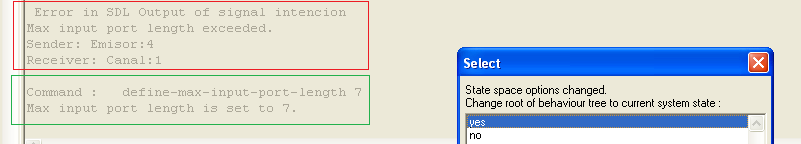
\includegraphics[width=0.95\linewidth]{src/error resuelto.png}
    \caption{\label{fig:errorresuelto} Error de máximo de puertos resuelto.}
\end{figure}

Se podrá explorar más el árbol y confirmar que no existen nuevos errores. Otra forma de visualización de los estados será usando el \textbf{MSC Tree}, aunque no nos centraremos mucho en ésta:

\quad 

\begin{figure}[h]
    \centering
    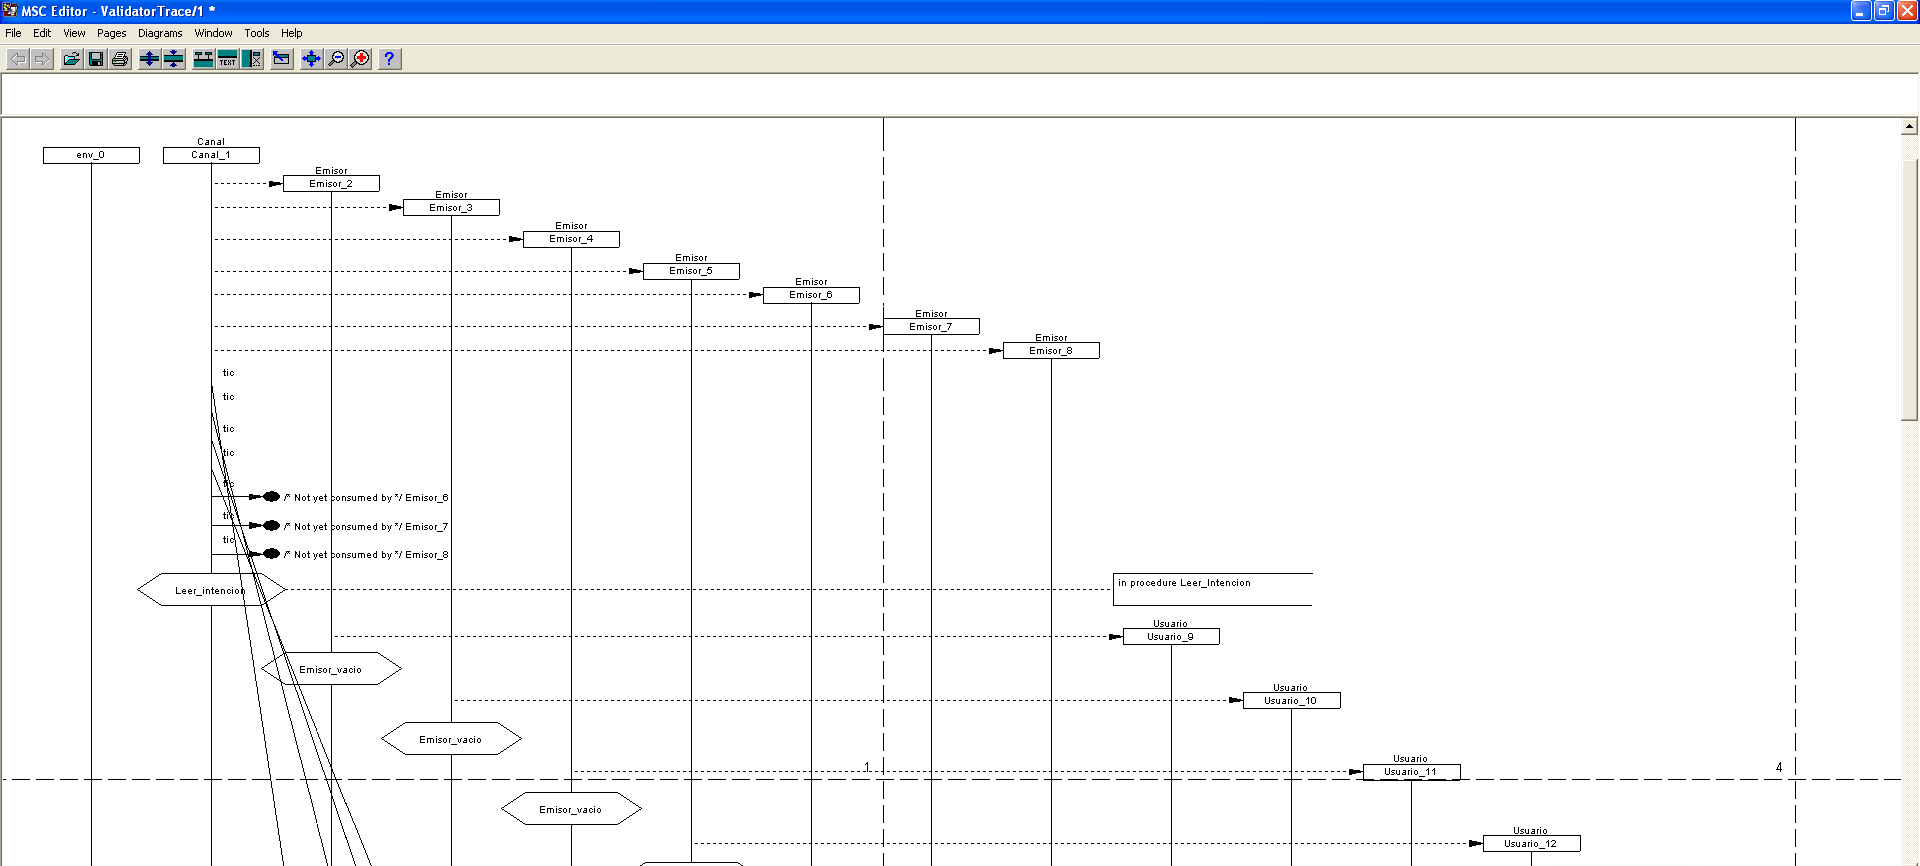
\includegraphics[width=0.65\linewidth]{src/MSC tree.png}
    \caption{\label{fig:msctree} Esquema de nuestro árbol MSC.}
\end{figure}

\subsection{Algoritmo Bit State}

Aunque anteriormente hayamos podido explorar los estados manualmente, existen algoritmos que nos pueden facilitar la \textbf{validación automática}, en este caso usaremos el \textbf{Algoritmo Bit State.}

El algoritmo de exploración Bit State se puede utilizar para validar sistemas SDL hasta un gran tamaño. Se representan los estados del sistema que se generan durante la exploración. Pulsaremos el botón \textbf{Bit State} en la UI de validación, y se realizará una primera exploración usando el algoritmo.

\quad 

Por defecto, tendremos un error, el cual será el mismo encontrado anteriormente, por lo que no podremos completar toda la cobertura de exploración. Para solucionarlo, lo haremos de la misma forma que antes usando \textbf{define-max-input-port-length 7.}

Hemos seleccionado un \textbf{max-input} de 7 y un \textbf{max-depth} de 1000. Podemos observar los datos obtenidos del algoritmo:
 
\begin{figure}[ht]
    \centering
    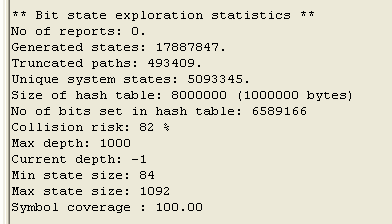
\includegraphics[width=0.65\linewidth]{src/bit state.png}
    \caption{\label{fig:bitstate} Estadísticas de la exploración Bit State.}
\end{figure}

\newpage

\section{Simulación}

Para la simulación manual desde \textbf{SIMULATOR UI} no haremos tanto inciso, ya que más adelante usaremos el archivo del simulador generado para realizar simulaciones automáticas por lotes. 

\quad

De todas formas, es necesario generar los archivos y comprobar la correcta simulación, por lo que iremos a \textbf{generate} $\rightarrow$ \textbf{make} $\rightarrow$ \textbf{fullmake}, habiendo seleccionado el standard kernel \textbf{Microsoft Simulation}. De este modo, se habrá generado un archivo \textbf{Aloha}\verb|_|\textbf{smc.exe}, el cual abriremos desde la interfaz del simulador. Tras esto, podremos proceder a la simulación desde un SMC Tree, y comprobamos que se pueda hacer de forma funcional.


\section{Obtención de datos y Análisis de los resultados}

Una vez se comprueba el funcionamiento de tanto la validación como la simulación, procederemos a obtener datos de varias simulaciones usando \textbf{MS-DOS.}

Primero probaremos con una simulación de prueba, donde únicamente se verá la simulación mediante la terminal de windows y no desde nuestra aplicación de Telelogic-tau. Abrimos el archivo generado por el kernel \textbf{Microsoft Simulation} anteriormente:

\quad

\begin{figure}[h]
    \centering
    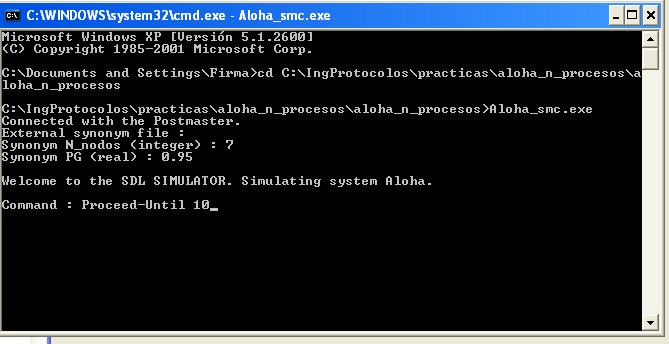
\includegraphics[width=0.85\linewidth]{src/cmd.png}
    \caption{\label{fig:cmdcaptura} Simulación de ALOHA mediante la terminal de windows.}
\end{figure}

Podemos observar que nos pide un archivo \textbf{synonym}, el cual no rellenaremos por el momento. También debemos de marcar los valores de las variables externas N\verb|_|nodos y PG, que como ya hemos comentado será de 7 y 0.95. El comando será de \textbf{Proceed-Until 10}, ya que de momento no necesitamos una gran simulación. Comprobamos que funcione correctamente. Para analizar los valores de las simulaciones, podremos usar el comando:


$$\verb|Command: Examine-Variable( Emisor 1 TOemisor )|$$

Cambiaremos \verb|Emisor 1| por el proceso que queramos observar, y \verb|TOemisor| por la variable cuyo dato queramos obtener.

\subsection{Simulación automática}

Hemos visto anteriormente cómo simular desde la terminal de Windows. Sabiendo esto, podemos aprovechar su funcionamiento para simular el mayor número de instancias con una sola ejecución.

\quad

Para ello, añadiremos nuestras variables y comandos a ejecutar en unos archivo que serán procesados en la simulación. Los llamaremos \textbf{siminit.syn} y \textbf{siminit.com}, y serán asignados como variable de entorno \textbf{SDTEXTSYNFILE}. Es importante utilizar las extensiones correctas, puesto que tienen el mismo nombre pero distinto contenido. En la ventana de comandos, usaremos:

$$\verb|set SDTEXTSYNFILE = siminit.syn|$$

Al archivo \textbf{siminit.syn} le añadiremos las variables externas:

\quad

\begin{center} 
    \begin{verbatim}
        N_nodos 7 
        PG 0.95
    \end{verbatim}
    \end{center} 
\quad

Y al archivo \textbf{siminit.com} le añadimos los comandos usados, sabiendo que tendremos 7 emisores:

\begin{center} 
    \begin{verbatim}

        set-trace 0
        Proceed-Until 10000
        Examine-Variable ( Canal S) 
        Examine-Variable ( Canal G) 
        Examine-Variable ( Emisor 1 TOemisor )
        Examine-Variable ( Emisor 2 TOemisor )
        Examine-Variable ( Emisor 3 TOemisor )
        Examine-Variable ( Emisor 4 TOemisor )
        Examine-Variable ( Emisor 5 TOemisor )
        Examine-Variable ( Emisor 6 TOemisor )
        Examine-Variable ( Emisor 7 TOemisor )
        Examine-Variable ( Emisor 1 TCemisor )
        Examine-Variable ( Emisor 2 TCemisor )
        Examine-Variable ( Emisor 3 TCemisor )
        Examine-Variable ( Emisor 4 TCemisor )
        Examine-Variable ( Emisor 5 TCemisor )
        Examine-Variable ( Emisor 6 TCemisor )
        Examine-Variable ( Emisor 7 TCemisor )
        Exit

    \end{verbatim}
    \end{center} 
\quad

Hemos preparado los archivos para la simulación automática, aunque haremos primero una prueba de una única simulación (con \textbf{Proceed-Until 10} para que no se alargue mucho) y lo guardaremos en un archivo para comprobar que funcionan éstos comandos, usaremos ahora en la ventana de comandos:

$$\verb|aloha_smc.exe > misresultados.txt|$$

Este archivo \textbf{ misresultados.txt} está guardado en la carpeta del trabajo. Comprobaremos ahora los datos con varias simulaciones. Se ejecutará un script batch en windows que contendrá un bucle recorriendo los datos que queremos obtener para distintos casos. Esto quiere decir que, haremos una simulación con \textbf{Proceed-Until-10000} para cada valor de PG que añadimos en el bucle for. Serán distintos valores de PG desde 0 hasta 0.95, que se guardarán en la carpeta \textbf{resultados}. Nuestro archivo \textbf{simular.bat} tendrá de contenido:
\begin{center} 
    \begin{verbatim}

        @echo off
        set SDTEXTSYNFILE=siminit.syn
        for %%i in (0 01 025 05 075 1 125 150 175 2 25 3
        35 4 45 5 6 7 8 9 95) do 
        (
        echo PG=0.%%i en fichero: resultado_0_%%i.txt
        echo N_nodos 7 > siminit.syn
        echo PG 0.%%i >> siminit.syn
        aloha_smc.exe > resultados\resultado_0_%%i.txt
        )

    \end{verbatim}
    \end{center} 
\quad

Tras un rato de simulación, tendremos los 21 archivos de texto en la carpeta \textbf{resultados}, ya podremos pasar a la parte final, que es el análisis de los mismos.

\subsection{Procesado de datos en Python}

Al generarse 21 archivos de texto, los datos se vuelven complicados de manejar, y copiar y pegar cada número del texto a Excel se haría muy repetitivo, por lo que haremos un script en Python que procese nuestros datos y genere las gráficas para los análisis. Primero tendremos que ver de qué forma podemos filtrar estos datos, la información de los archivos será de esta forma:

\begin{center} 
    \begin{verbatim}

        No connection with the Postmaster. Running stand-alone.
        Using external synonym file "siminit.syn" according to environment 
        variable "SDTEXTSYNFILE".
        
        Welcome to the SDL SIMULATOR. Simulating system Aloha.
        
        Command : set-trace 0
        Default trace set to 0
        
        Command : 
        
        Command : Proceed-Until 10000
        
        Command : Examine-Variable ( Canal S) 
        S (integer) = 3082
        
        Command : Examine-Variable ( Canal G) 
        G (integer) = 18245
        
        Command : Examine-Variable ( Emisor 1 TOemisor )
        TOemisor (integer) = 2563
        
        Command : Examine-Variable ( Emisor 2 TOemisor )
        TOemisor (integer) = 2619
        .                   .                       .
        . (resto del texto) .                       .
        .                   .                       .
        Command : Examine-Variable ( Emisor 7 TStotal )
        TStotal (integer) = 4189
        
        Command : Exit
        Simulation terminated

    \end{verbatim}
    \end{center} 
\quad

Procedemos a crear el archivo \textbf{main.py} que se encontrará en la carpeta \textbf{resultados}, y para inicializar tendremos que hacer un bucle que recorra todos nuestros archivos \verb|resultado_0_X.txt|, lo haremos con un array que contenga los valores de PG y lo sumaremos al nombre (La almohadilla "\verb|#|" se usa para comentarios en python y no modificar el código):

\quad 
\begin{center} 
    \begin{verbatim}

    valores = ["0", "01", "025","05", "075", "1", "125", "150", "175",
    "2", "25", "3", "35", "4", "45", "5", "6", "7", "8", "9", "95"]

    # Iteramos nuestro array de valores, "valor" será cada número de dentro
    for valor in valores:

        # sumamos resultado_0_ a valor y luego ".txt":
        archivo = "resultado_0_" + valor + ".txt"

        with open(archivo, 'r') as file: # Abrimos el archivo

    \end{verbatim}
    \end{center} 
\quad

Ahora que tenemos un archivo por cada iteración, buscaremos una forma para filtrar el texto innecesario del txt, viendo el contenido del texto de antes, podemos observar que en las líneas que aparecen los números que nos interesan, aparece la palabra \verb|integer|, por lo que nos quedaremos únicamente con esas líneas:

\begin{center} 
    \begin{verbatim}

    lines = []

    # Iteramos las líneas del archivo una por una
    for line in file:

        # Si la línea contiene "integer" nos quedamos con ella:
        if "integer" in line:

            # "rstrip" elimina los espacios de sobra
            line = line.rstrip()

            # "append" añade la línea en la que estamos al array lines
            lines.append(line)

    \end{verbatim}
    \end{center} 

Si ejecutamos el código que llevamos hasta el momento, podremos ver las líneas que han sido filtradas, aunque no sea el resultado que buscamos hemos reducido el texto que sobra:

\quad

\begin{figure}[h]
    \centering
    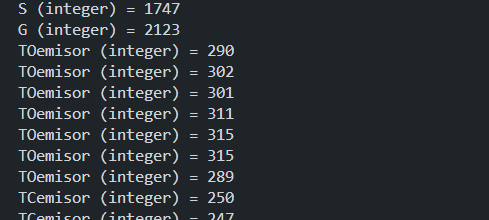
\includegraphics[width=0.7\linewidth]{src/lineas filtradas1.png}
    \caption{\label{fig:filtradas1} Líneas filtradas en el Script.}
\end{figure}

Falta guardar esos números en un array correspondiente para cada nombre, pero se añade un nuevo problema, ahora no sabemos para qué emisor es cada línea (Es decir, aparece TOemisor pero no si es el 1,2,3...). Para solucionar esto, contaremos el número de líneas equivalentes al archivo de texto original, de modo que nuestra línea filtrada 1 será la S, la 2 la G, de la 3 a la 9 irán los TO de 1 al 7, de la 10 a la 16 los TC, y así con las demás. Una vez contado eso, declararemos los arrays correspondientes y filtraremos únicamente el número que haya en la línea, de modo que nuestra línea pasaría a ser esto:

$$\verb|TOemisor (integer) = 290| \rightarrow 290$$

E iteramos cada línea filtrada. Según el número de la línea, lo añadiremos al array TOemisor, o a los demás. Cabe destacar que además de añadir estos valores al array, también sumaremos el valor a unas variables que hemos declarado como \textbf{valoresTO, valoresTC, valoresTS y valoresTP}. Nos servirá para luego dividirlas entre 10000, que nos dará la media que también la añadiremos al final de cada array de TOemisor, TCemisor... 

Vemos el código necesario para el filtrado del número concreto y añadirlo a nuestros arrays:

\quad 

\begin{center} 
    \begin{verbatim}

    # bucle con las líneas ya filtradas
    for i in range(len(lines)):

        # string será nuestra línea filtrada
        string = lines[i]

        # Match será un valor booleano que busca un dígito. \d significa int
        match = re.search(r'\d+', string)

        # Esto es como decir if match == True en python
        if match:

            # Guardamos el número y lo pasamos a int
            numero_str = match.group()
            numero_int = int(numero_str)

            # Añadimos a los arrays según la línea que sea
            if i==0:
                S = numero_int
            elif i==1:
                G = numero_int
            elif i>1 and i<=8:
                TOemisor.append(numero_int)
                valoresTO = valoresTO + numero_int
            elif i>8 and i<=15:
                TCemisor.append(numero_int)
                valoresTC = valoresTC + numero_int
            elif i>15 and i<=22:
                TPemisor.append(numero_int)
                valoresTP = valoresTP + numero_int
            else:
                TStotal.append(numero_int)
                valoresTS = valoresTS + numero_int
    \end{verbatim}
    \end{center} 
\quad

Con esto tendremos los valores filtrados en un array de cada tipo, podemos ejecutar el Script para ver lo que llevamos hasta ahora:

\begin{figure}[h]
    \centering
    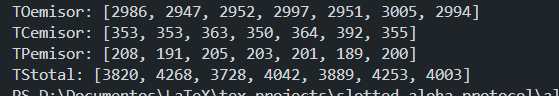
\includegraphics[width=0.7\linewidth]{src/lineas filtradas2.png}
    \caption{\label{fig:filtradas2} Datos en los arrays de cada tipo.}
\end{figure}

Ya tenemos lo importante, y como hemos visto anteriormente, estábamos iterando a su vez para cada archivo, esto sigifica que se guardaría un array de TOemisor, TCemisor, TPemisor, y TStotal para cada valor de PG. Cada array lo guardaremos al final de cada iteración en una posición de las listas que crearemos como \textbf{TOemisores, TCemisores, TPemisores y TStotales}, de modo que tendremos un array de arrays, donde cada posición de éste sería un valor de PG, (o un archivo diferente de \verb|resultado_0_X.txt|). Dicho de otra forma, tendríamos una matriz. Ésto es lo que buscamos para exportarlo a un archivo como \textbf{Excel}.

\quad

Antes de exportar nuestros datos a Excel, declararemos alguna variable y añadiremos al principio de cada fila el valor de PG, y al final el valor de la media (ValoresTO/10000), todo esto se puede ver en el archivo completo: \textbf{main.py} en la carpeta \textbf{resultados}.

Exportamos a Excel:

\begin{center} 
    \begin{verbatim}

    # DataFrame será como el equivalente a la matriz, le añadimos los títulos 
    df_TOemisores = pd.DataFrame(TOemisores, columns=["PG", "TOemisor1",
     "TOemisor2", "TOemisor3", "TOemisor4", "TOemisor5", "TOemisor6",
      "TOemisor7", "Media TO"])

    # Exportamos a xlsx
    with pd.ExcelWriter("datos_filtrados.xlsx") as writer:

        # Escribir el DataFrame de TOemisores en la primera hoja
        df_TOemisores.to_excel(writer, sheet_name='TOemisores', index=False)

    \end{verbatim}
    \end{center} 
\quad

Añadiremos las matrices restantes a las diferentes hojas del archivo \verb|datos_filtrados.xlsx|. Con esto se habría terminado de procesar los datos.

\begin{figure}[h]
	\centering
	\begin{subfigure}{0.5\textwidth}
		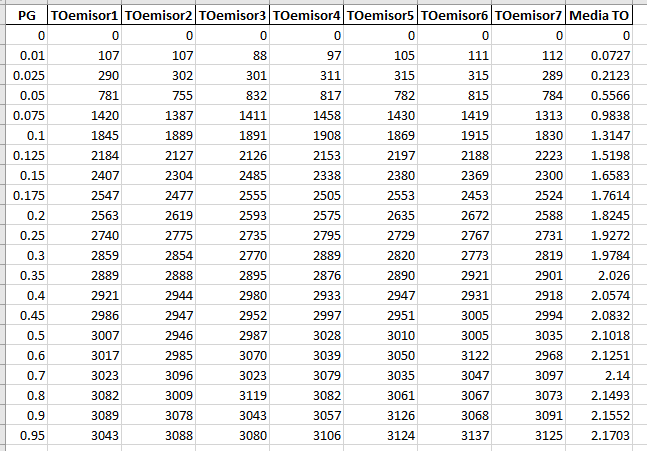
\includegraphics[width=\linewidth]{src/TOemisor.png}
		\caption{Hoja TOemisor}
		\label{fig:TOemisorcsv}
	\end{subfigure}%
	\begin{subfigure}{0.5\textwidth}
		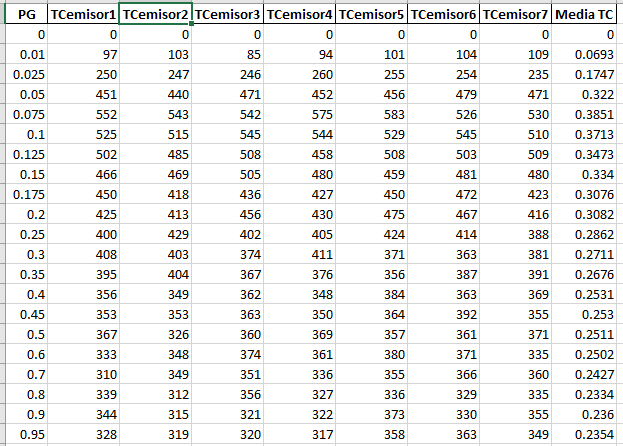
\includegraphics[width=\linewidth]{src/TCemisor.png}
		\caption{Hoja TCemisor}
		\label{fig:TCemisorcsv}
	\end{subfigure}
	\caption{}
	\label{fig:Ambastablas}
\end{figure}

\begin{figure}[h]
	\centering
	\begin{subfigure}{0.5\textwidth}
		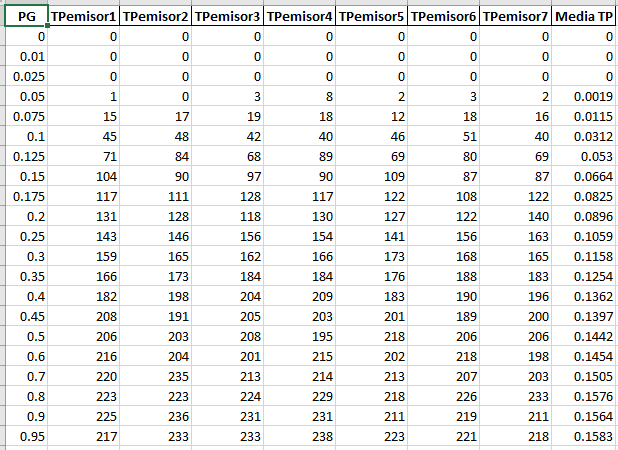
\includegraphics[width=\linewidth]{src/TPemisor.png}
		\caption{Hoja TPemisor}
		\label{fig:TPemisorcsv}
	\end{subfigure}%
	\begin{subfigure}{0.5\textwidth}
		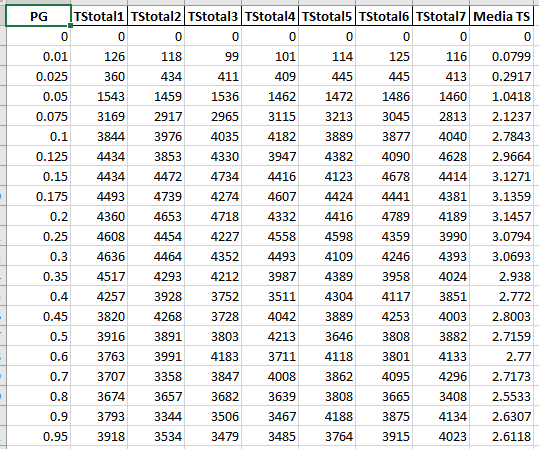
\includegraphics[width=\linewidth]{src/TStotal.png}
		\caption{Hoja TStotal}
		\label{fig:TStotalcsv}
	\end{subfigure}
	\caption{}
	\label{fig:Ambastablas2}
\end{figure}

Una vez tenemos los datos guardados, como ya tenemos los datos en DataFrames, podremos generar las gráficas con las medias de éstos (últimas columnas).

\subsection{Generar gráficas en Python}

Haremos un nuevo Script para generar las gráficas, vamos a aprovechar que los datos están guardados en DataFrames para evitar el uso de Excel. El archivo será \textbf{generarGraficas.py}, donde importará las variables que nos hacen falta del archivo \textbf{main.py}, y usaremos un módulo para generar las gráficas, matplotlib. De esta forma, las gráficas serán:
\newpage
\begin{figure}[h]
    \centering
    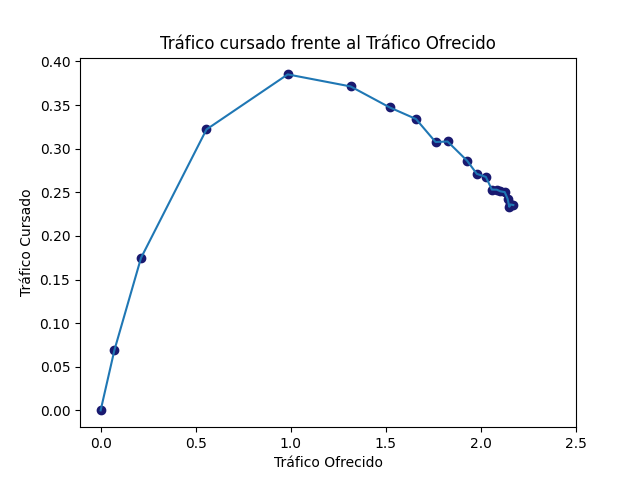
\includegraphics[width=0.7\linewidth]{src/TCvsTO.png}
    \caption{\label{fig:TCvsTO} Datos en los arrays de cada tipo.}
\end{figure}

En esta primera gráfica, estamos comparando el Tráfico Cursado frente al Tráfico Ofrecido, que nos muestra la curva de eficiencia del canal. Podríamos obtener un valor óptimo cuando el Tráfico Ofrecido se aproxima a 1, despreciando el Tráfico perdido por el momento. Vemos como mayor Tráfico Ofrecido no implica mayor Tráfico Cursado.

\begin{figure}[h]
    \centering
    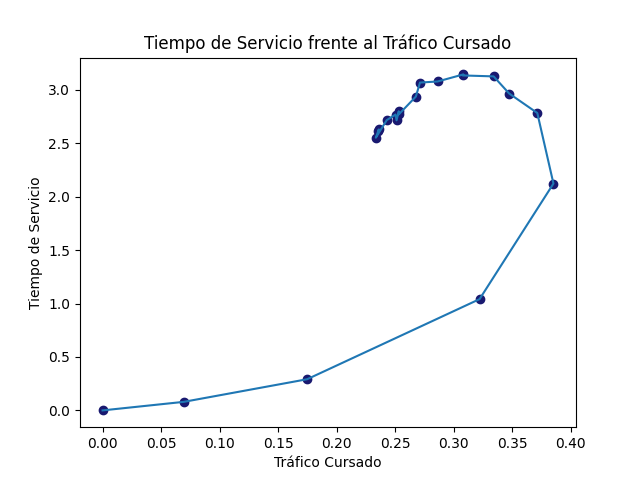
\includegraphics[width=0.7\linewidth]{src/TSvsTC.png}
    \caption{\label{fig:TSvsTC} Datos en los arrays de cada tipo.}
\end{figure}

En la segunda gráfica, comparamos el Tiempo de servicio frente al Tráfico Cursado, que nos muestra el tiempo medio de Servicio. Se puede observar que a partir de ciertos valores, el tiempo de servicio pasa a ser exponencial.

\begin{figure}[h]
    \centering
    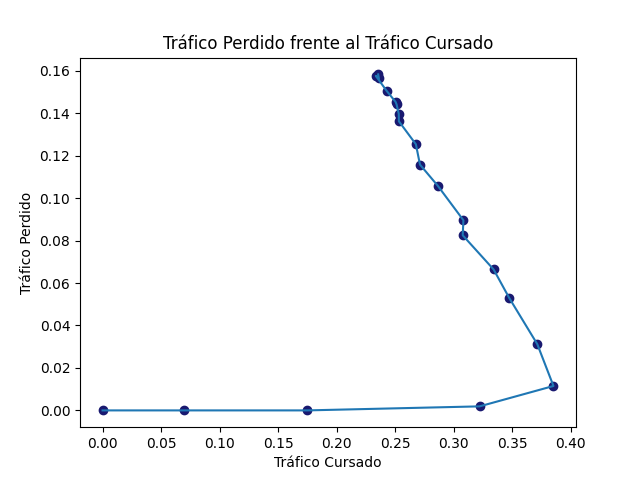
\includegraphics[width=0.7\linewidth]{src/TPvsTC.png}
    \caption{\label{fig:TPvsTC} Datos en los arrays de cada tipo.}
\end{figure}

Aquí compararemos el Tráfico Perdido frente al Tráfico Cursado,que nos muestra el número de paquetes perdidos. De la misma forma que en el tiempo medio de servicio, los paquetes perdidos aumentarían de forma exponencial. 

\begin{figure}[h]
	\centering
	\begin{subfigure}{0.5\textwidth}
		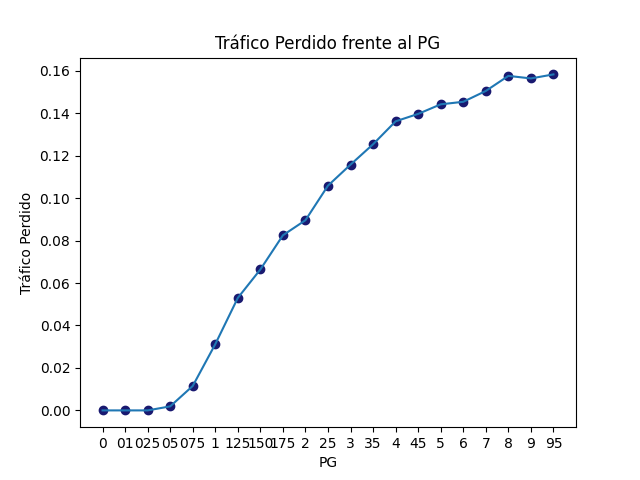
\includegraphics[width=\linewidth]{src/TPvsPG.png}
		\caption{}
		\label{fig:TPvsPG}
	\end{subfigure}%
	\begin{subfigure}{0.5\textwidth}
		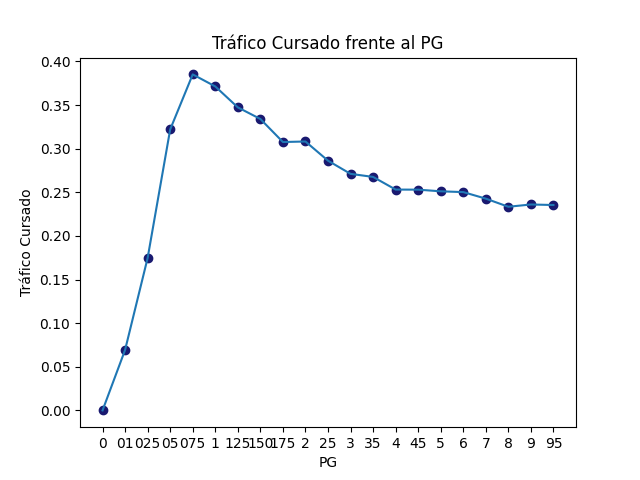
\includegraphics[width=\linewidth]{src/TCvsPG.png}
		\caption{}
		\label{fig:TCvsPG}
	\end{subfigure}
	\caption{Valores de TP y TC frente a PG}
	\label{fig:PGgraficas}
\end{figure}

Para finalizar, añadiremos dos últimas gráficas ya que al tener un script que nos genere las gráficas, los datos se hacen más manejables. Observamos tanto el Tráfico Perdido y el Tráfico Cursado para los valores distintos de PG, donde PG es la probabilidad de transmisión de un paquete. 

\quad

El Tráfico Perdido aumenta en relación al aumento de PG, algo esperable debido a que aumenta la probabilidad de colisión, aunque hay valores al inicio donde no parece afectar demasiado. Con el Tráfico Cursado pasa parecido, conforme aumenta el PG, disminuye el Tráfico que se cursa, aunque ésto solo pasa a partir de un valor, que es el cuando \textbf{PG = 0.075}, hasta ese valor el Tráfico Cursado tiene tendencia ascendente. 

Es por es que, para el valor de PG 0.075, obtenemos un valor de Tráfico Cursado Óptimo (Entre 0.30 y 0.40), el Tráfico Perdido no es grande, pero según la \hyperref[fig:TSvsTC]{\textbf{Figura 22}}, el tiempo de servicio, en esos valores alcanzan un tiempo de servicio bastante alto.

\quad

En conclusión, \textbf{0.075} puede ser el valor óptimo de nuestro sistema, dependiendo de lo que se busca en función del rendimiento, si se asume una ligera subida del tiempo de servicio, todo esto para 7 nodos.

\end{document}